This thesis presents a number of novel approaches to the analysis of spike trains. Mathematical neuroscience is a new and active field of applied mathematics which uses many different mathematical concepts to model the behaviour of the brain.  Spike train analysis deals with mathematical idealisations of the voltage trace of individual neurons, which are called spike trains.



\section{Spike trains}

Neurons convey information through the nervous system by generating
electric pulses which propagate along nerve fibers.  These pulses are
called action potentials or spikes \cite{DuBoisReymond1884a}. 

A typical cortical neuron has a resting potential of approximately -70 mV relative to
its surroundings, the cell is said to be polarised at this point.
The membrane potential of a neuron is affected by current
flowing into its synapses from other neurons, most of which make the membrane potential less negative, but the potential tends back towards the resting potential
unless the it nears a certain threshold. If a neuron
is depolarised so that its membrane potential is raised above this
threshold, the neuron generates an action potential. An action potential, or 
spike, is a rapid depolarisation and repolarisation of the membrane potential, a fluctuation in the membrane potential which typically lasts 
approximately 1ms. Following the production of a spike the neuron briefly 
becomes hyperpolarised, and as such cannot generate a spike for the next
couple of milliseconds.  This period, when a spike cannot be fired, is
called the absolute refractory period of a neuron.  Since the neuron
becomes hyperpolarised by the spike, there is also a period in which
it is more difficult for the neuron to spike again, this is called
the relative refractory period of a neuron. 

\begin{figure}[htb]
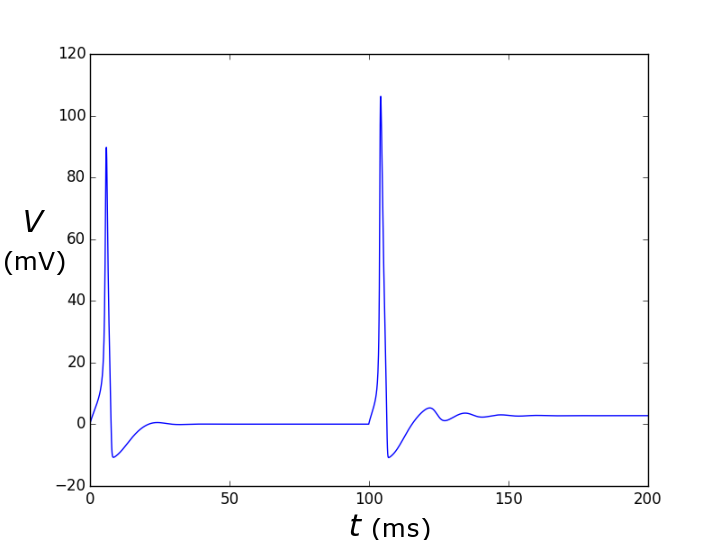
\includegraphics[width=\textwidth]{hhtrace}
\caption{The voltage trace of a pair of spikes generated by the Hodgkin-Huxley model.  Simulation run using the python package Brian \cite{GoodmanBrette2008a}}
\end{figure}

The dynamics of the membrane potential were precisely modelled in \cite{HodgkinHuxley1952a} by modelling the flow of sodium and potassium ions into and out of the neuron.  Their model was based on the voltage traces that they recorded from the giant axon in a squid \cite{HodgkinHuxley1939a}, but has proven to be the standard against which other neuron models are judged \cite{Izhikevich2004a}.

Spikes are very important because they propagate over long distances without 
attenuation, and so are the way in which neurons communicate with one another 
throughout the nervous system.  While there is some variation in 
the duration, amplitude and shape of action potentials, for a single neuron they typically exhibit a characteristic voltage trace as discussed in \cite{Lewicki1998a}. The spike then can be represented by choosing a particular point of the typical action potential, thus the timing of the spikes give much of the information.  So, 
if a neuron spikes $n$ times in a certain trial, then the trial can be 
described by the times of the spikes $t_i$.  The 
\emph{spike train} can then be described mathematically as:
\begin{equation}
s(t) = \sum_{i=1}^n \delta(t-t_i).
\end{equation}
The $\delta$ here is the Dirac delta, which gives a spike a volume equal to 
one at the point $t_i$.

\subsection{Spike train metrics}

While observing spike trains from a specific neuron, ideally one would be able to 
\lq{}decode\rq{} them and be able to describe the stimulus which evoked them.  
This is a very difficult problem, so the first step towards this problem is to try to distinguish which spike trains amongst a collection were evoked by 
the same stimulus.  There are several {\sl metrics} in the 
literature which give a ``distance'' between two spike trains.  

In Mathematics a metric space is a space equipped with a scalar function which gives a  
``distance'' between two elements in the space, called a \emph{metric}.  A metric is a function on a set 
$X$, $d: X\times X \rightarrow [0,\infty )$ that follows  
intuition for what a distance should be. That is, distances are non-negative, 
symmetric and only zero if two elements are the same. The Triangle Inequality 
states that you should never be able to shorten the distance between two points 
by going through an intermediate point, so it is the notion that the shortest 
distance between two points is a straight line.


\subsection{van Rossum metric}

The metric proposed in 
\cite{VanRossum2001a}, is based on the $L^2$ metric on function 
spaces.  If spike trains are viewed as sums of Dirac delta functions, 
then by convolving the spike trains, $s(t)$, with 
a kernel, $k(t)$, each spike train can be represented in a real function space.  A common kernel that is used is the exponential kernel
\begin{equation}
k(t) = \left\{ \begin{array}{ll}\frac{1}{\tau}e^{-\frac{t}{\tau}}, & t\geq 0 \\
0, & t<0\end{array} \right. .
\end{equation}

\begin{figure}[htb]
% GNUPLOT: LaTeX picture with Postscript
\begingroup
  \makeatletter
  \providecommand\color[2][]{%
    \GenericError{(gnuplot) \space\space\space\@spaces}{%
      Package color not loaded in conjunction with
      terminal option `colourtext'%
    }{See the gnuplot documentation for explanation.%
    }{Either use 'blacktext' in gnuplot or load the package
      color.sty in LaTeX.}%
    \renewcommand\color[2][]{}%
  }%
  \providecommand\includegraphics[2][]{%
    \GenericError{(gnuplot) \space\space\space\@spaces}{%
      Package graphicx or graphics not loaded%
    }{See the gnuplot documentation for explanation.%
    }{The gnuplot epslatex terminal needs graphicx.sty or graphics.sty.}%
    \renewcommand\includegraphics[2][]{}%
  }%
  \providecommand\rotatebox[2]{#2}%
  \@ifundefined{ifGPcolor}{%
    \newif\ifGPcolor
    \GPcolorfalse
  }{}%
  \@ifundefined{ifGPblacktext}{%
    \newif\ifGPblacktext
    \GPblacktexttrue
  }{}%
  % define a \g@addto@macro without @ in the name:
  \let\gplgaddtomacro\g@addto@macro
  % define empty templates for all commands taking text:
  \gdef\gplbacktext{}%
  \gdef\gplfronttext{}%
  \makeatother
  \ifGPblacktext
    % no textcolor at all
    \def\colorrgb#1{}%
    \def\colorgray#1{}%
  \else
    % gray or color?
    \ifGPcolor
      \def\colorrgb#1{\color[rgb]{#1}}%
      \def\colorgray#1{\color[gray]{#1}}%
      \expandafter\def\csname LTw\endcsname{\color{white}}%
      \expandafter\def\csname LTb\endcsname{\color{black}}%
      \expandafter\def\csname LTa\endcsname{\color{black}}%
      \expandafter\def\csname LT0\endcsname{\color[rgb]{1,0,0}}%
      \expandafter\def\csname LT1\endcsname{\color[rgb]{0,1,0}}%
      \expandafter\def\csname LT2\endcsname{\color[rgb]{0,0,1}}%
      \expandafter\def\csname LT3\endcsname{\color[rgb]{1,0,1}}%
      \expandafter\def\csname LT4\endcsname{\color[rgb]{0,1,1}}%
      \expandafter\def\csname LT5\endcsname{\color[rgb]{1,1,0}}%
      \expandafter\def\csname LT6\endcsname{\color[rgb]{0,0,0}}%
      \expandafter\def\csname LT7\endcsname{\color[rgb]{1,0.3,0}}%
      \expandafter\def\csname LT8\endcsname{\color[rgb]{0.5,0.5,0.5}}%
    \else
      % gray
      \def\colorrgb#1{\color{black}}%
      \def\colorgray#1{\color[gray]{#1}}%
      \expandafter\def\csname LTw\endcsname{\color{white}}%
      \expandafter\def\csname LTb\endcsname{\color{black}}%
      \expandafter\def\csname LTa\endcsname{\color{black}}%
      \expandafter\def\csname LT0\endcsname{\color{black}}%
      \expandafter\def\csname LT1\endcsname{\color{black}}%
      \expandafter\def\csname LT2\endcsname{\color{black}}%
      \expandafter\def\csname LT3\endcsname{\color{black}}%
      \expandafter\def\csname LT4\endcsname{\color{black}}%
      \expandafter\def\csname LT5\endcsname{\color{black}}%
      \expandafter\def\csname LT6\endcsname{\color{black}}%
      \expandafter\def\csname LT7\endcsname{\color{black}}%
      \expandafter\def\csname LT8\endcsname{\color{black}}%
    \fi
  \fi
  \setlength{\unitlength}{0.0500bp}%
  \begin{picture}(7200.00,5040.00)%
    \gplgaddtomacro\gplbacktext{%
      \csname LTb\endcsname%
     % \put(462,3863){\makebox(0,0)[r]{\strut{} 0}}%
      %\put(462,4231){\makebox(0,0)[r]{\strut{} 1}}%
      %\put(462,4599){\makebox(0,0)[r]{\strut{} 2}}%
      \put(594,3580){\makebox(0,0){\strut{} 0}}%
      \put(1836,3580){\makebox(0,0){\strut{} 0.02}}%
      \put(3078,3580){\makebox(0,0){\strut{} 0.04}}%
      \put(4319,3580){\makebox(0,0){\strut{} 0.06}}%
      \put(5561,3580){\makebox(0,0){\strut{} 0.08}}%
      \put(6803,3580){\makebox(0,0){\strut{} 0.1}}%
      \put(3698,4929){\makebox(0,0){\strut{}(a)}}%
    }%
    \gplgaddtomacro\gplfronttext{%
    }%
    \gplgaddtomacro\gplbacktext{%
      \csname LTb\endcsname%
      \put(462,2183){\makebox(0,0)[r]{\strut{} 0}}%
      \put(462,2551){\makebox(0,0)[r]{\strut{} 1}}%
      \put(462,2919){\makebox(0,0)[r]{\strut{} 2}}%
      \put(594,1900){\makebox(0,0){\strut{} 0}}%
      \put(1836,1900){\makebox(0,0){\strut{} 0.02}}%
      \put(3078,1900){\makebox(0,0){\strut{} 0.04}}%
      \put(4319,1900){\makebox(0,0){\strut{} 0.06}}%
      \put(5561,1900){\makebox(0,0){\strut{} 0.08}}%
      \put(6803,1900){\makebox(0,0){\strut{} 0.1}}%
      \put(3698,3249){\makebox(0,0){\strut{}(b)}}%
    }%
    \gplgaddtomacro\gplfronttext{%
    }%
    \gplgaddtomacro\gplbacktext{%
      \csname LTb\endcsname%
      \put(462,503){\makebox(0,0)[r]{\strut{} 0}}%
      \put(462,749){\makebox(0,0)[r]{\strut{} 1}}%
      \put(462,994){\makebox(0,0)[r]{\strut{} 2}}%
      \put(462,1240){\makebox(0,0)[r]{\strut{} 3}}%
      \put(594,220){\makebox(0,0){\strut{} 0}}%
      \put(1836,220){\makebox(0,0){\strut{} 0.02}}%
      \put(3078,220){\makebox(0,0){\strut{} 0.04}}%
      \put(4319,220){\makebox(0,0){\strut{} 0.06}}%
      \put(5561,220){\makebox(0,0){\strut{} 0.08}}%
      \put(6803,220){\makebox(0,0){\strut{} 0.1}}%
      \put(3698,1570){\makebox(0,0){\strut{}(c)}}%
        \put(3698,10){\makebox(0,0){\strut{} $t$ (s)}}%
    }%
    \gplgaddtomacro\gplfronttext{%
    }%
    \gplbacktext
    \put(0,0){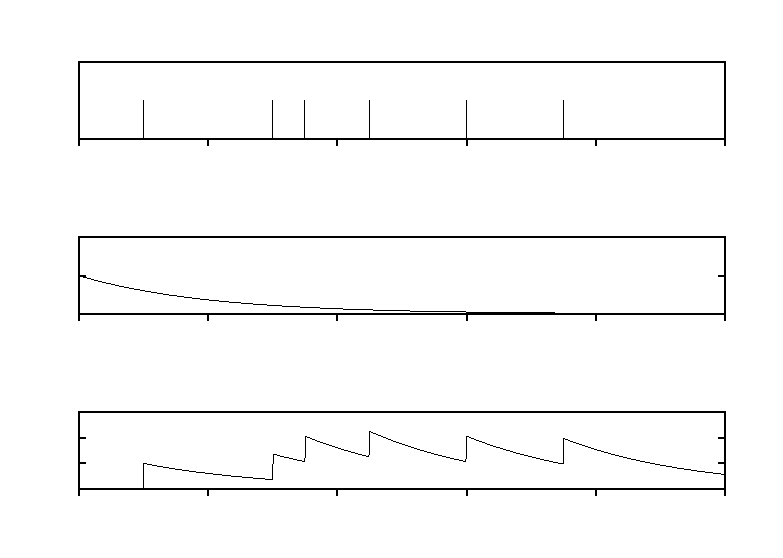
\includegraphics{vRfilter}}%
    \gplfronttext
  \end{picture}%
\endgroup

\caption{\label{stk} Shown above is an example of the filtering process of the van Rossum metric.  A sample spike train (a) is convolved with an exponential filter (b), where the timescale $\tau=20$ ms, to get the function $u(t)$ (c).}
\end{figure}

This kernel the advantage of computability over a 
gaussian kernel.  So, we get a new function $u(t)$ after convolving the spike 
train with the kernel:
\begin{equation}
u(t) = s*k(t) = \int_0^T s(t-s)k(s)\,ds
\end{equation}



%\begin{figure}[tb]
%  \centering
%  \includegraphics[width=0.8\textwidth]{spiketrainkernel.eps}
%  \rule{35em}{0.5pt}
%  \caption{This figure shows  an exponential kernel (a), which we convolve with a spike train (b), to get the function (c) which represents the spike train.  We take the  $L^2$-metric between such functions to get the van Rossum metric between spike trains.}
%  \label{stk}
%\end{figure}

Figure \ref{stk} above shows the form of the function that is produced by
convolving a spike train with the exponential kernel.  The metric is then simply the $L_2$ distance between pairs of these functions, $u$ and $v$ say, that is:
\begin{equation}
d(u,v) = \sqrt{\int_0^T (u(t) - v(t))^2\,dt}.
\end{equation}
It has been shown that once the correct timescale has been chosen the choice of kernel has 
little effect on the performance of this metric \cite{PaivaParkPrincipe2010}.

\subsection{Victor-Purpura metric}

In \cite{VictorPurpura1997a} another metric is described.  This type of metric is called an \lq{}edit-length\rq{} metric, as it is based on a theoretical \lq{}cost\rq{} of transforming one spike-train to another.  The fundamental principle is that each transformation has a non-zero cost, so by minimising over all transformations which transform one spike train, $X$ say, into another, $Y$.

There are three different permitted fundamental transformations.  It is possible to insert a spike at any time, which has a cost of one.  Similarly, any spike can be deleted for a cost of one.  The third permitted transformation is to move a spike $\Delta t$, which has a cost $q\Delta t$, for some timescale parameter $q>0$.

Then the Victor-Purpura metric between two spike trains, $X$ and $Y$, is the minimum over all combinations of fundamental functions which transform $X$ to $Y$.  This can be written as:
\begin{equation}
d_{\text{VP}}(X,Y) = \min_f \sum_i c\left( f_i(X) \right)
\end{equation}
where $f=f_1\circ\ldots\circ f_m$ is a function such that $f(X) = Y$.

This is obviously a metric. There is a non-zero cost for each transformation, so $d(X,Y)=0$ only if $X=Y$. Since insertion and deletion are symmetric operations, it is clear that $d(X,Y)=d(Y,X)$.  Then the triangle equality follows, since if $f$ transforms $X$ to $Y$, and $g$ transforms $Y$ to $Z$, then $h=g\circ f$ must transform $X$ to $Z$, and since the Victor-Purpura metric requires that the minimum cost, $h$ must have cost greater than or equal to $d(X,Z)$.

\subsection{SPIKE distance}
In \cite{KreuzEtAl2011a} a distance measure was proposed, which does not require a time-scale parameter and which can also be used as a time-local measure of spike train synchrony.

The 

\section{Information Theory}
Information Theory has been used widely in Computational Neuroscience, eg. to compare spike trains \cite{BialekEtAl1998a} and to try to determine the information content of spike-trains\cite{GillespieHoughton2009a}.

The topic of Information Theory is centred around the definition of \emph{entropy}, provided by Shannon in 1948 \cite{Shannon1948a}.  Entropy is a measure of the information content of a random variable $X$, with observations $x \in \mathcal{X}$ and probability distribution $p:\mathcal{X} \rightarrow [0,1]$, it is defined as:
\begin{equation}
H(X) = -\sum_{x\in\mathcal{X}}  p(x) \log_2 p(x)
\end{equation}
Entropy is measured in \emph{bits}, so the entropy of a random variable can be viewed as the minimum number of binary bits required to efficiently code the random variable.